\documentclass[aspectratio=43,10pt]{beamer}
\usetheme{UniBern}

%\usepackage{eso-pic}
%\usepackage{transparent}
%\newcommand\BackgroundPic{%
%	\put(0,0){%
%		\parbox[b][\paperheight]{\paperwidth}{%
%			\vfill
%			\centering
%			{\transparent{0.25}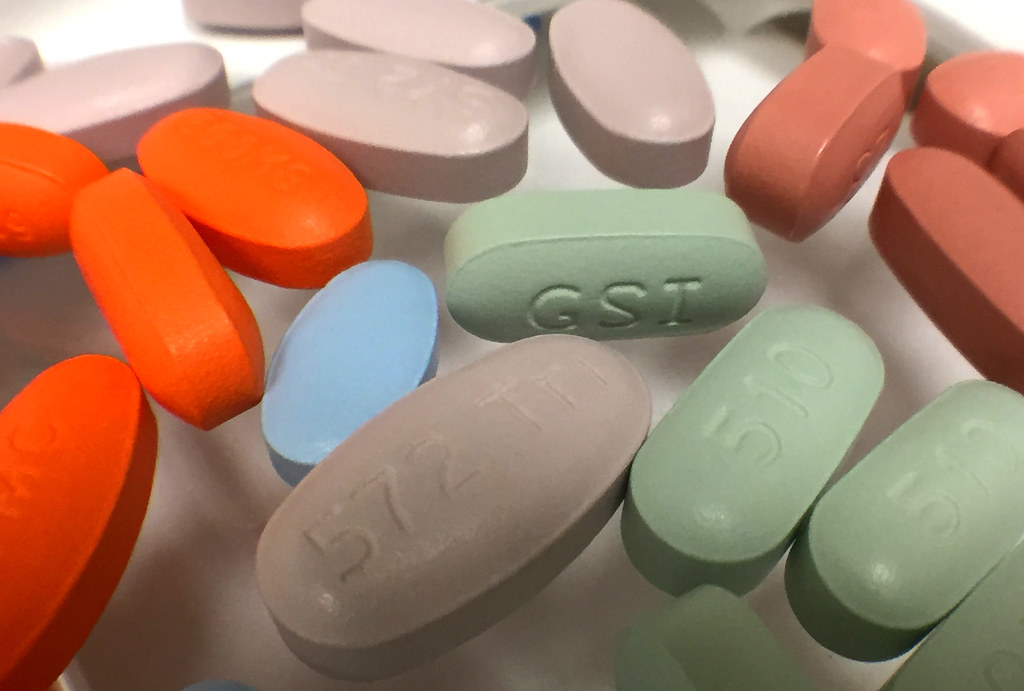
\includegraphics[width=1.2\paperwidth,height=1.2\paperheight,keepaspectratio]{pills.jpg}}
%			\vfill
%}}}

\usepackage{tikz}
\usepackage{dsfont}

\definecolor{maroon}{RGB}{176, 48, 96}
\definecolor{orange2}{RGB}{255, 165, 0}
\newcommand{\colindic}[1]{\textcolor{maroon}{#1}}
\newcommand{\colsurvey}[1]{\textcolor{orange2}{#1}}

\title{The heterogeneous rise of HIV drug resistance in Southern Africa}
\author{\underline{Julien Riou}, Matthias Egger, Christian Althaus}
\institute{Institute of Social and Preventive Medicine (ISPM) \\ \vspace{.3em} University of Bern, Switzerland}
\date{Stancon 2019, Cambridge UK}



\begin{document}
	
%	\AddToShipoutPicture*{\BackgroundPic}

\frame{
\maketitle
}

\frame{
	\frametitle{HIV in Africa}

	\begin{figure}
	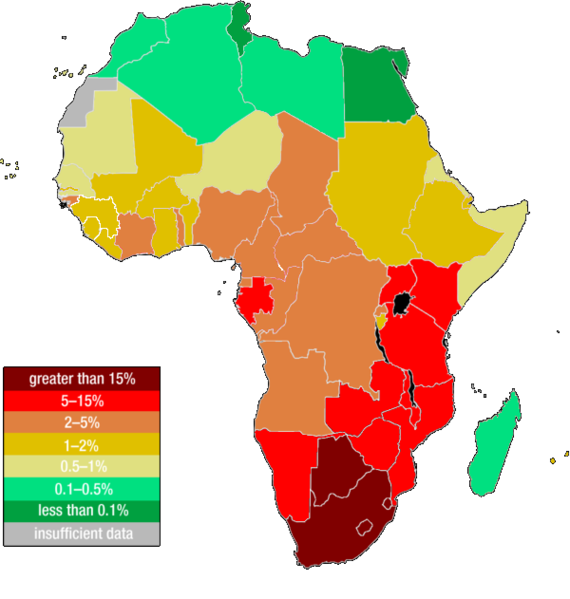
\includegraphics[width=.55\textwidth]{hiv_africa.png}
	\vspace{-1.5em}
	\caption{Proportion of persons living with HIV Africa in 2017 (UNAIDS)}	
	\end{figure}
}

\frame{
	\frametitle{ART roll-out since the early 2000s}
	\vspace{-1.5em}
	\begin{figure}
		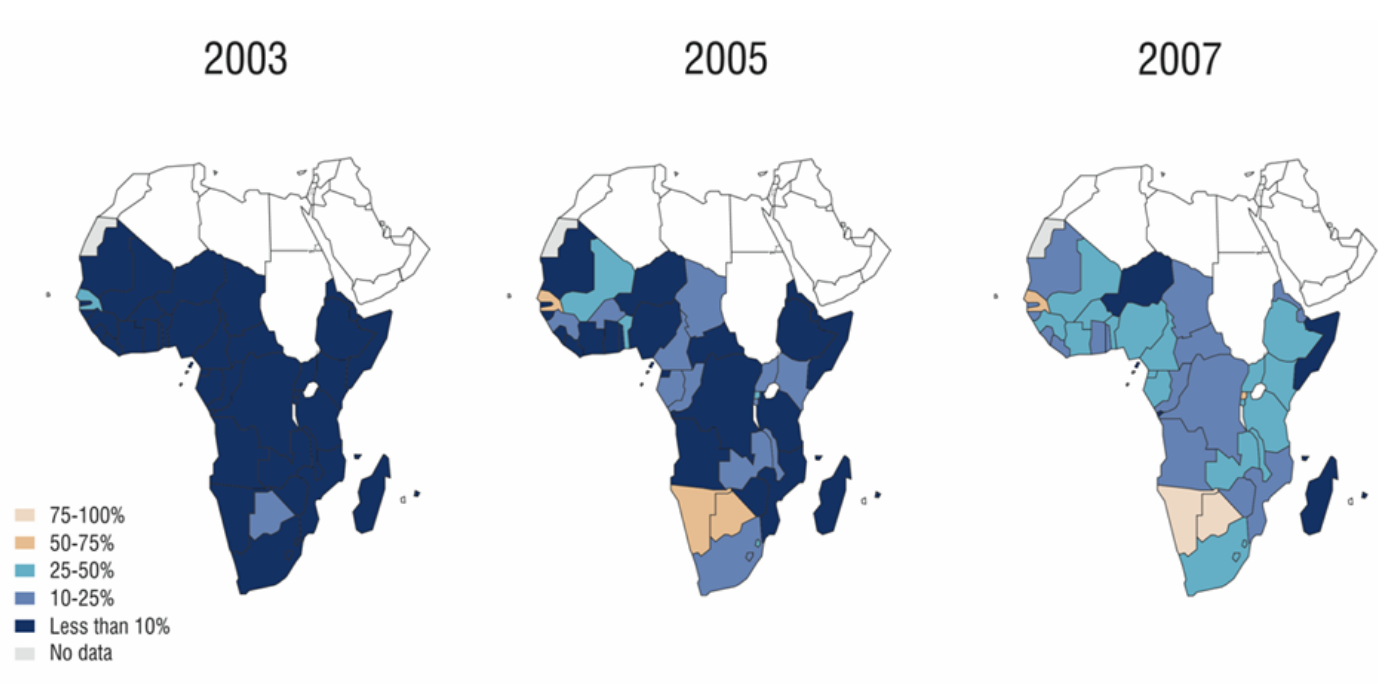
\includegraphics[width=.92\textwidth]{hiv_art.png}
		\vspace{-1em}
		\caption{Proportion of person living with HIV on antiretroviral therapy (UNAIDS)}	
	\end{figure}

	Combination \alert{antiretroviral therapy} (ART):
	\begin{itemize}
		\item 2 nucleoside analog reverse-transcriptase inhibitors (\alert{NRTI})
		\item 1 non-nucleoside reverse-transcriptase inhibitor (\alert{NNRTI})
	\end{itemize}
}

\frame{
	\frametitle{NNRTI resistance}
	HIV resistance to \alert{NNRTI} poses a growing threat to the success of ART:
	\vspace{.2em}
	\begin{itemize}
		\item low genetic barrier to resistance\footnote{Stanford University, HIV drug resistance database} 
		% single mutation resulting in complete loss of drug activity
		\item poor adherence, bad prescription practices, supply chains...
	\end{itemize}
	\vspace{2em}\pause
	
	Assessed by monitoring \alert{pretreatment drug resistance} (PDR): 
	\vspace{.2em}
	\begin{itemize}
		\item resistance mutations measured at the moment of treatment initiation
		\item acquired by transmission
	\end{itemize}

}
\frame{
	\frametitle{Growing NNRTI resistance in Africa}
	Systematic review of PDR surveys in adults\footnote{Gupta et al. (\textit{The Lancet Infectious Diseases}, 2017)}:\vspace{1em}
	\begin{figure}[h]
		\begin{tikzpicture}
		\node[anchor=south west,inner sep=0] at (0,0) {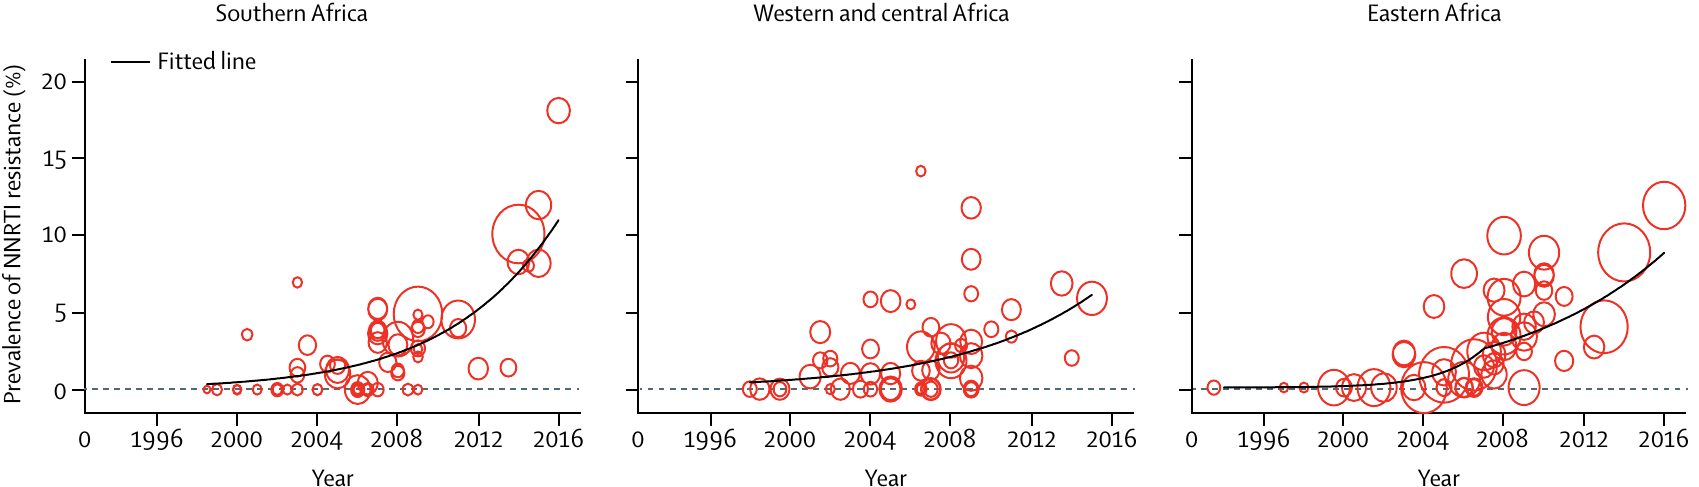
\includegraphics[width=\textwidth]{../figures/gupta_2017_fig1.png}};
		\node[gray] (SA) at (2,2.4) {{\tiny $+23\%~[16-29]$}} ;
		\node[gray] (WA) at (6,2.4) {{\tiny $+17\%~[6-29]$}} ;
		\node[gray] (EA) at (10,2.4) {{\tiny $+11\%~[2-20]$}} ;
		\end{tikzpicture}
		\vspace{-1em}
		\caption{NNRTI PDR by year of sampling (\textcolor{gray}{yearly increase in odds of PDR})\textsuperscript{3}}	
	\end{figure}
%	\vspace{.2em}
	\centering\alert{$\Rightarrow$ Descriptive analysis of the evolution of PDR by continental region}
	\vspace{1.5em}
}


\frame{
	\frametitle{Comments}	
		Regional estimates may mask large between-country \alert{heterogeneity}\vspace{1em}
		
	\pause The level of resistance in a population is dependent on \alert{ART uptake}:\vspace{.2em}
		\begin{itemize}
			\item especially relevant for between-country comparison
			\vspace{.2em}
			\item timing and scale of ART roll-out differ by country
		\end{itemize}
	\begin{figure}
		\includegraphics[width=.75\textwidth]{../figures/plot_desc_art.pdf}
		\vspace{-1.5em}
		\caption{Proportion of person living with HIV on ART in Southern Africa (UNAIDS)}	
	\end{figure}
	
%	The \alert{national scale} might be better suited to monitor NNRTI resistance:
%	\vspace{.2em}
%	\begin{itemize}
%		\item PDR is directly dependent on the timing and scale of ART roll-out
%		\vspace{.2em}
%		\item public health policies are conducted at the national level
%	\end{itemize}
%	\vspace{.5em}
%	\begin{figure}
%		\includegraphics[width=.75\textwidth]{../figures/plot_desc_art.pdf}
%		\vspace{-1.5em}
%		\caption{Proportion of PLHIV on ART in Southern Africa (UNAIDS)}	
%	\end{figure}
 }

%\frame{
%	\frametitle{Comments (2)}
%	PDR only gives a \alert{partial picture} of NNRTI resistance:
%	\vspace{.2em}
%	\begin{itemize}
%		\item delay between infection with a resistant strain and ART initiation\vspace{.1em}
%		\item dependence on the transmission dynamics of HIV \vspace{.1em}
%%		\item differential transmission of resistant strains: \vspace{.1em}
%%		\begin{itemize}
%%			\item individuals on ART have very low transmissibility\footnote{Supervie et al. (\textit{CID}, 2014)}\vspace{.1em}
%%			\item resistance favors ART failure and thus higher transmissibility\vspace{.1em}
%%			\item no fitness cost of resistance regarding transmission\footnote{Kühnert et al. (\textit{PLoS Pathogens}, 2018)} \vspace{.1em}
%%		\end{itemize}
%		\item \alert{non-linear} association with the overall prevalence of resistance\vspace{2em}
%	\end{itemize}
%}


\frame{
	\frametitle{Reanalysis for Southern Africa}
	\vspace{-2em}
	\begin{figure}[h]
		\begin{tikzpicture}
		\node[anchor=south west,inner sep=0] at (0,0) {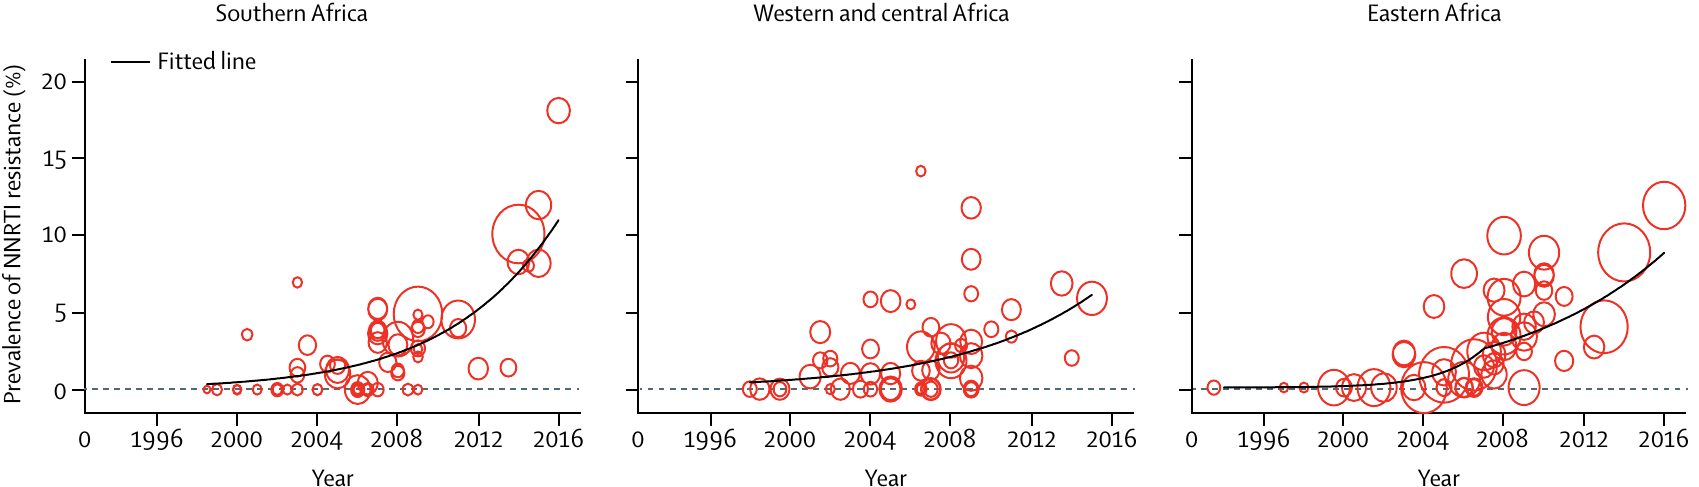
\includegraphics[width=\textwidth]{../figures/gupta_2017_fig1.png}};
		\node[gray] (SA) at (2,2.4) {{\tiny $+23\%~[16-29]$}} ;
		\node[gray] (WA) at (6,2.4) {{\tiny $+17\%~[6-29]$}} ;
		\node[gray] (EA) at (10,2.4) {{\tiny $+11\%~[2-20]$}} ;
		\draw[white] (-0.1,3.4) rectangle ++(4.2,-3.6);
		\draw[ubRed, rounded corners] (-0.1,3.4) rectangle ++(4.2,-3.5);
		\end{tikzpicture}
	\end{figure}
	\textit{Objectives:} \vspace{.2em}
	\begin{enumerate}
		\item develop a \alert{mechanistic} model describing the processes leading to PDR (mutation, transmission, treatment, measurement in surveys)\pause
		\item \alert{account} for the main characteristics of HIV transmission and treatment\pause
		\item in \alert{every country} of Southern Africa 
	\end{enumerate}\vspace{.4em}

%		$\Rightarrow$ \textit{at the crossroads of statistical inference and infectious disease modelling }
}


\frame{
	\frametitle{Modelling strategy}
		
	We want a \alert{multivariate model} able to fit jointly, in each country:
	
	\vspace{0.5em}
	\begin{tabular}{p{8cm}|l}
		\hspace{1em}\alert{$\bullet$} the adult prevalence of HIV $(\colindic{\mathds{A}})$ & \\
		\hspace{1em}\alert{$\bullet$} the number of HIV-infected adults under ART  $(\colindic{\mathds{B}})$ &\colindic{UNAIDS} \\			
		\hspace{1em}\alert{$\bullet$} the AIDS-related mortality $(\colindic{\mathds{C}})$ & \\
		\hspace{1em}\alert{$\bullet$} the size of the adult population $(\colindic{\mathds{D}})$ & \\
%		\hspace{1em}\alert{$\bullet$} the adult incidence of HIV $(\colindic{\mathds{D}})$ & \\
%		\hspace{1em}\alert{$\bullet$} the number of AIDS-related adult deaths $(\colindic{\mathds{E}})$ & \\

	\end{tabular}
	\vspace{.6em}
	
	\begin{tabular}{p{8cm}|l}
		\hspace{1em}\alert{$\bullet$} pretreatment drug resistance in adults $(\colsurvey{\mathds{E}})$ & \colsurvey{Systematic review} \\
	\end{tabular}

	\vspace{1.5em}\pause

	E.g. for the Republic of South Africa (RSA):
	\vspace{-.3em}
	\begin{figure}
		\includegraphics[height=2.8cm]{../figures/indicators_data.pdf}
		\includegraphics[height=2.8cm]{../figures/pdr_data.pdf}
	\end{figure}
}

\frame{
	\frametitle{Model 1}
	Starting with a simple system of ODEs:
	\begin{figure}
	\scalebox{.8}{\begin{tikzpicture}
		\node (NULL) at (0,-2.5) { };
		\node (NULL2) at (9,.5) { };
		\only<1>{
			\scalebox{1.25}{
		\node[anchor=west] (C1) at (1.5,0) {$\frac{dS}{dt}=-\beta S I$};
		\node[anchor=west] (C2) at (1.5,-.65) {$\frac{dI}{dt}=\beta S I - \tau \mathbf{1}_{\tau}(t,t_0)I$};
		\node[anchor=west] (C3) at (1.5,-1.3) {$\frac{dR}{dt}=\tau \mathbf{1}_{\tau}(t,t_0)I$};

	}}
		\only<2->{
		\node[circle, draw, inner sep=0pt, minimum size=1cm] (S) at (0,0) {$S$};
		\node[circle, draw, inner sep=0pt, minimum size=1cm] (I) at (4,0) {$I$};
		\node[circle, draw, inner sep=0pt, minimum size=1cm] (T) at (8,0) {$T$};
		
		\draw[->,>=latex] (S) edge node[above] {$\beta S I$} (I);
		\draw[->,>=latex] (I) edge node[above] {$\tau \mathbf{1}_{\tau}(t,t_0)I$} (T);
			}
		\only<3->{
		\node[draw,rectangle,rounded corners,fill=maroon!10,text width=2.4cm, text centered] (A) at (4,-1.8) {{\small Prevalence:} ${a_t} = I(t) + T(t)$};
		\draw[dashed,maroon] (I) -- (A);
		\draw[dashed,maroon] (T) -- (A);
		\node[draw,rectangle,rounded corners,fill=maroon!10,text width=1.8cm, text centered] (B) at (8,-1.8) {{\small Treated:} ${b_t} = T(t)$};
		\draw[dashed,maroon] (T) -- (B);
		}	
		\end{tikzpicture}}
	\end{figure}

	\vspace{1.5em}

	With the step function $\mathbf{1}_{\tau}(t,t_0)$ depending on the year of ART roll-out $t_0$:
	$$
	\mathbf{1}_{\tau}(t,t_0) = \begin{cases} 
	0 & \text{if} \ \ t<t_0 \\
	1 & \text{otherwise}
	\end{cases}
	$$
		\vspace{1.5em}
		Initial values 	$S(0), I(0), T(0)$ are set using data from 2000
	
}


\frame{
	\frametitle{Model 1}
			\vspace{-1.5em}
	We fit the model to yearly estimates of HIV prevalence (\colindic{$\mathds{A}$}) and of the number of adults on ART (\colindic{$\mathds{B}$})
	using independent \alert{normal distributions}\footnote{after variance-stabilizing square-root transformation, see Yu (\textit{Stat. \& Prob. Letters}, 2009)}:	\vspace{.5em}
 	$$ \Pr\left(\begin{bmatrix}\sqrt{\colindic{\mathds{A}_t}} \\ \sqrt{\colindic{\mathds{B}_t}}\end{bmatrix} \ \middle| \ \beta, \tau, \sigma_a, \sigma_b \right)  = \mathcal{N}\left( \begin{bmatrix}\sqrt{\colindic{{a}_t}} \\ \sqrt{\colindic{{b}_t}}\end{bmatrix}, \begin{bmatrix}\sigma^2_a & 0 \\ 0 & \sigma^2_b \end{bmatrix}  \right) $$
	
	\vspace{1.2em}
		\small{
			\begin{tabular}{l|l}
				where:  &  $\beta$ is the parameter governing transmission \\
						& $\tau$ is the parameter governing treatment initiation \\
				 &  $\sigma_a$ and $\sigma_b$ are the error parameters related to  \colindic{$\mathds{A}$} and \colindic{$\mathds{B}$} \\
				 & $\begin{bmatrix}\colindic{{a}_t} \\ \colindic{{b}_t}\end{bmatrix} = g(\beta, \tau, t, t_0) $ is the \alert{output of the ODE system} at time $t$ \\
			\end{tabular}
		}
}

\frame{
	\frametitle{Model 1}
	We choose \alert{weakly informative priors} for all parameters:
	$$ \beta \sim \text{Expon}(5) \hspace{2em} \tau \sim \text{Expon}(5) \hspace{2em} \sigma_a \sim \text{Expon}(1) \hspace{2em} \sigma_b \sim \text{Expon}(1) $$
	\pause
	We check the adequacy of these choices by \alert{simulating from the priors}\only<2>{\footnote{Gabry et al. (\textit{Journal of the Royal Statistical Society}, 2019)}}:
	\begin{figure}
		\includegraphics[width=.8\textwidth]{../figures/prior_indicators_L1.pdf}
		\vspace{-1em}
		\caption{\textit{Prior predictive check}\textsuperscript{7} for model 1 in the RSA}
	\end{figure}
}



\frame{
	\frametitle{Model 1}
	We fit the model in \texttt{Stan} and get the following \alert{posterior distributions}:
		\begin{figure}
		\begin{tikzpicture}
		\node[anchor=south west,inner sep=0] at (0,0) {\includegraphics[width=.8\textwidth]{../figures/post_params_L1.png}};
		\fill[color=orange,fill opacity=.4] (7.7,0) rectangle (9.25,1.58);
		\end{tikzpicture}
	\end{figure}

	\pause	That correspond to the following \alert{fit}:
	
	\begin{figure}
		\includegraphics[width=.8\textwidth]{../figures/post_indicators_L1.pdf}
		\vspace{-1em}
		\caption{Fit of model 1 to \colindic{$\mathds{A}$} and \colindic{$\mathds{B}$} (in RSA) }
	\end{figure}
}


\frame{
	\frametitle{Model 2}
	\vspace{1em}
	We improve the adequacy of the model to the \alert{non-linear rise} of the number of adults on ART by replacing the step function by a logistic function:
		\vspace{.2em}
	$$ \mathbf{1}_{\tau}(t,t_0,\nu,\xi) = \frac{1}{1+e^{-\xi (t-t_0-\nu)}} $$ 
	
	\vspace{.4em}
	\small{\begin{tabular}{l|l}
		where: & $t_0$ is the year of ART roll-out in the country (here 2004)\\
		& $\xi$ is a logistic growth rate (i.e. the steepness)\\
		& $\nu$ is a shift in years (i.e. time to reach 50\% of maximum) \\
		\end{tabular}
	}
	\vspace{.4em}\pause
	\begin{figure}
		\hspace{-2em}\includegraphics[width=.4\textwidth]{../figures/plot_modelM2_tau.pdf}
		\vspace{-1.6em}
		\caption{Prior predictive check on the \alert{effective treatment rate}, i.e. $\tau \mathbf{1}_{\tau}(t,t_0,\nu,\xi)$}
	\end{figure}
}

\frame{
	\frametitle{Model 2}
	We follow the same procedure and obtain:
	\begin{figure}
		\begin{tikzpicture}
\node[anchor=south west,inner sep=0] at (0,0) {\includegraphics[width=.8\textwidth]{../figures/post_params_L2.png}};
\only<1>{\fill[fill=orange,fill opacity=.4] (9.25,1.6) rectangle (0,1.3);}
\only<2>{\fill[fill=orange,fill opacity=.4] (9.25,1.35) rectangle (0,1.05);}
\only<3>{\fill[fill=orange,fill opacity=.4] (9.25,1.08) rectangle (0,0.55);}

\end{tikzpicture}
	\end{figure}
	
	\begin{figure}
		\includegraphics[width=.9\textwidth]{../figures/post_indicators_L2.pdf}
		\vspace{-1em}
		\caption{Fit of model 2 to \colindic{$\mathds{A}$} and \colindic{$\mathds{B}$} (in RSA) }
	\end{figure}
}


\frame{
	\frametitle{Model 3}
	We add population \alert{growth} and AIDS-related \alert{mortality}:
	\vspace{-2.9em}
	\begin{figure}
		\scalebox{.8}{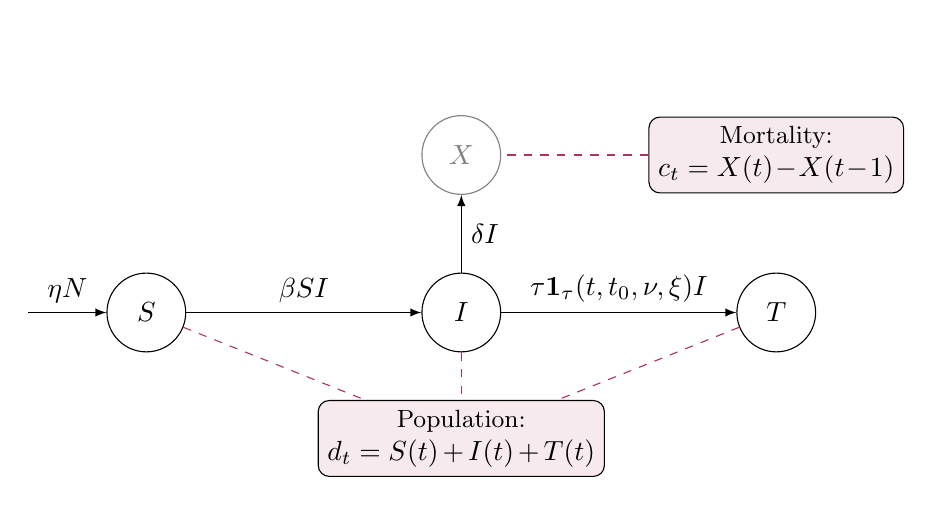
\begin{tikzpicture}
			\node[circle, draw, inner sep=0pt, minimum size=1cm] (S) at (0,0) {$S$};
			\node[circle, draw, inner sep=0pt, minimum size=1cm] (I) at (4,0) {$I$};
			\node[circle, draw, inner sep=0pt, minimum size=1cm] (T) at (8,0) {$T$};
			\node[circle, draw, inner sep=0pt, minimum size=1cm,white] (E1) at (4,2) { };
			\node[circle, draw, inner sep=0pt, minimum size=1cm,white] (E2) at (8,2) { };
			\node (NULL) at (9,3.5) { };
			
			\draw[->,>=latex] (S) edge node[above] {$\beta S I$} (I);
			\draw[->,>=latex] (I) edge node[above] {$\tau \mathbf{1}_{\tau}(t,t_0,\nu,\xi)I$} (T);
			\draw[->,>=latex] (-1.5,0) -- (S) node[midway,above] {$\alert{\eta} N$};
			\draw[->,>=latex] (I) -- (E1) node[midway,right] {$\alert{\delta} I$};
			\pause
			\node[circle, draw, inner sep=0pt, minimum size=1cm,gray] (D2) at (4,2) { $X$ };	
			\node[draw,rectangle,rounded corners,fill=maroon!10,text width=3cm, text centered] (D3) at (8,2) {{\small Mortality:}\\ ${c_t} = X(t) - X(t-1) $};
			\draw[dashed,maroon] (D3) -- (D2);

			\pause
			\node[draw,rectangle,rounded corners,fill=maroon!10,text width=3.4cm, text centered] (C) at (4,-1.6) {{\small Population:} \\ ${d_t} = S(t) + I(t) + T(t)$};
			\draw[dashed,maroon] (S) -- (C);
			\draw[dashed,maroon] (I) -- (C);
			\draw[dashed,maroon] (T) -- (C);
			\end{tikzpicture}}
	\end{figure}
	\vspace{.2em}
	\small{\begin{tabular}{l|l}
		where: & $\eta$ is the rate of growth of the adult population \\
		& $\delta$ is the death rate among untreated HIV-infected individuals\\
	\end{tabular}
}
}

\frame{
	\frametitle{Model 3}
	\begin{figure}
		\begin{tikzpicture}
\node[anchor=south west,inner sep=0] at (0,0) {\includegraphics[width=.8\textwidth]{../figures/post_params_L3.png}};
\only<1>{\fill[fill=orange,fill opacity=.4] (9.25,2.65) rectangle (0,1.58);}
\only<2>{\fill[fill=orange,fill opacity=.4] (9.25,1.6) rectangle (0,1.3);}
\only<3>{\fill[fill=orange,fill opacity=.4] (9.25,1.35) rectangle (0,1.05);}


\end{tikzpicture}
	\end{figure}
	\vspace{-.5em}
	\begin{figure}
		\includegraphics[width=.9\textwidth]{../figures/post_indicators_L3.pdf}
		\vspace{-1.5em}
		\caption{Fit of model 3 to \colindic{$\mathds{A}$}, \colindic{$\mathds{B}$}, \colindic{$\mathds{C}$} and \colindic{$\mathds{D}$} (in RSA) }
	\end{figure}
}

\frame{
	\frametitle{Model 4}	
			\vspace{-2em}
		Occurrence and transmission of \alert{NNRTI resistance}:
		\vspace{-1.5em}
		\begin{figure}
		\begin{center}
		\scalebox{.7}{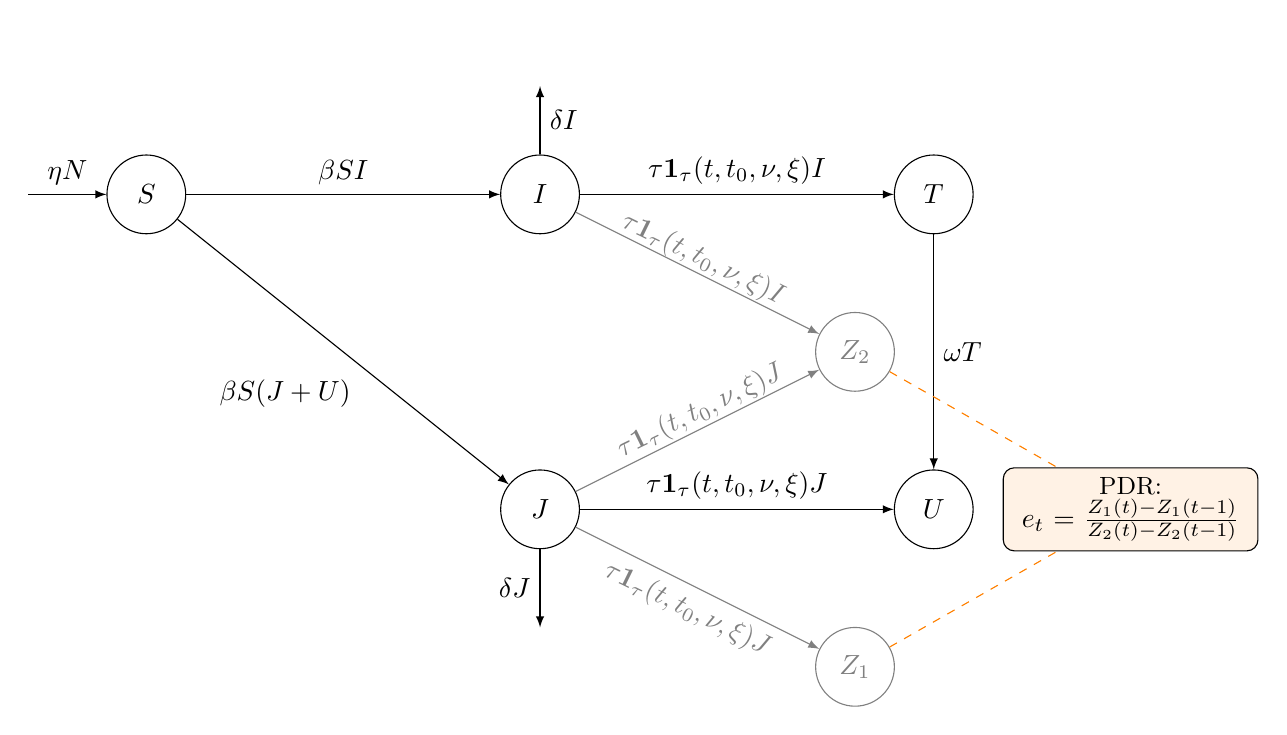
\begin{tikzpicture}
			% cascade of care
			\node[circle, draw, inner sep=0pt, minimum size=1cm] (S) at (0,2) {$S$};
			\node[circle, draw, inner sep=0pt, minimum size=1cm] (I) at (5,2) {$I$};
			\node[circle, draw, inner sep=0pt, minimum size=1cm] (T) at (10,2) {$T$};
			\node (E1) at (5,3.5) { };
			\node (E2) at (13.5,-4.1) { };
			\node (E3) at (13.5,4) { };

			\draw[->,>=latex] (S) edge node[above] {$\beta S I$} (I);
			\draw[->,>=latex] (I) edge node[above] {$\tau \mathbf{1}_{\tau}(t,t_0,\nu,\xi)I$} (T);
			\draw[->,>=latex] (-1.5,2) -- (S) node[midway,above] {$\eta N$};
			\draw[->,>=latex] (I) -- (E1) node[midway,right] {${\delta} I$};
		   	% resistance among disease failure
			\pause
			\node[circle, draw, inner sep=0pt, minimum size=1cm] (U) at (10,-2) {$U$};
			\draw[->,>=latex] (T) edge node[right] {$\alert{\omega} T$} (U);
			\pause
			% resistance transmission
			\node[circle, draw, inner sep=0pt, minimum size=1cm] (J) at (5,-2) {$J$};
			\draw[->,>=latex] (S) edge node[xshift=-21,yshift=-15] {$\beta S (\alert{J+U})$} (J);
			\pause
			\draw[->,>=latex] (J) edge node[above] {$\tau \mathbf{1}_{\tau}(t,t_0,\nu,\xi)J$} (U);
			% mortality
			\pause
		    \draw[->,>=latex] (J) -- ++(0,-1.5) node [left, pos=0.5] {$\delta J$};
			\pause
			\node[circle, draw, inner sep=0pt, minimum size=1cm,gray] (Z2) at (9,0) { $Z_2$ };	
			\draw[->,>=latex,gray] (I) edge node[xshift=2,yshift=5,rotate=-26]{$\tau \mathbf{1}_{\tau}(t,t_0,\nu,\xi)I$} (Z2);
			\draw[->,>=latex,gray] (J) edge node[xshift=1,yshift=7, rotate=26]{$\tau \mathbf{1}_{\tau}(t,t_0,\nu,\xi)J$} (Z2);
			\pause
			\node[circle, draw, inner sep=0pt, minimum size=1cm,gray] (Z1) at (9,-4) { $Z_1$ };	
			\draw[->,>=latex,gray] (J) edge node[below, rotate=-26]{$\tau \mathbf{1}_{\tau}(t,t_0,\nu,\xi)J$} (Z1);

			\pause
			\node[draw,rectangle,rounded corners,fill=orange!10,text width=3cm, text centered] (F) at (12.5,-2) {{\small PDR:} \\ ${e_t} = \frac{Z_1(t)-Z_1(t-1)}{Z_2(t)-Z_2(t-1)}$};
			\draw[dashed,orange] (Z1) -- (F);
			\draw[dashed,orange] (Z2) -- (F);

		\end{tikzpicture}}
		\end{center}
		\end{figure}
	\only<9>{We also add a parameter $\iota$ for the \alert{initial proportion of resistance} (in 2000)}
}

\frame{
	\frametitle{Model 4}
	In addition to the indicators $\{\mathds{\colindic{A}, \colindic{B}, \colindic{C}, \colindic{D}}\}$, we also fit the model to \alert{survey data}: 
	$$ \Pr(\colsurvey{\mathds{E}_i} |\theta) = \text{Binom}(\mathds{N}_i, \colsurvey{e_i}) $$
	{\small \begin{tabular}{l|l}
			where: & $\colsurvey{\mathds{E}_i}$ is the number of individuals with NNRTI resistance in study $i$ \\
			& $\theta = \{ \beta,\tau,\nu,\xi,\delta,\eta,\omega,\iota,\sigma_{a,\ldots,d}\}$ represents all 12 parameters  \\
			& $\mathds{N}_i$ is the sample size of study $i$ \\
			& $\colsurvey{e_i} = g(\theta,t=\mathds{T}_i,t_0)$ is the model-predicted PDR at the time of survey $i$\\
	\end{tabular}}
	\pause\vspace{2.5em}

	So that the full likelihood is:
	$$ \Pr(\mathds{\colindic{A}, \colindic{B}, \colindic{C},\colindic{D}, \colsurvey{E}} | \theta) = \prod_{t,i} \Pr(\colindic{\mathds{A}_t},\colindic{\mathds{B}_t},\colindic{\mathds{C}_t},\colindic{\mathds{D}_t}| \theta ) \Pr(\colsurvey{\mathds{E}_i} | \theta)$$
	 
}

\frame{
	\frametitle{Model 4}
	\vspace{-1em}
	\begin{figure}
		\begin{tikzpicture}
		\node[anchor=south west,inner sep=0] at (0,0) {\includegraphics[width=.8\textwidth]{../figures/post_params_L4.png}};
\only<1>{\fill[fill=orange,fill opacity=.4] (9.25,3.15) rectangle (0,1.55);}
\only<2>{\fill[fill=orange,fill opacity=.4] (9.25,1.6) rectangle (0,1.05);}

		\end{tikzpicture}
%		\includegraphics[width=.8\textwidth]{../figures/post_params_L4.png}
	\end{figure}
	\vspace{0em}
		\begin{figure}
		\includegraphics[width=.8\textwidth]{../figures/post_indicators_L4.pdf}
			\vspace{-1.5em}
		\caption{Fit of model 4 to \colindic{$\mathds{A}$}, \colindic{$\mathds{B}$}, \colindic{$\mathds{C}$} and \colindic{$\mathds{D}$} (in RSA) }
	\end{figure}
}

\frame{
	\frametitle{Model 4}
	\vspace{-1em}
	\begin{figure}
		\includegraphics[width=.7\textwidth]{../figures/post_pdr_L4.pdf}
		\vspace{-1em}
		\caption{Fit of model 4 to \colsurvey{$\mathds{E}$} (in RSA) }
	\end{figure}
}

\frame{
	\frametitle{Model 4M}
	We now extend model 4 to the \alert{9 countries} of the region:
	\begin{itemize}
		\item independence for the parameters related to the local dynamics of HIV
		$$ \{\beta_k, \tau_k, \nu_k, \xi_k, \eta_k, \delta_k,\sigma_{a,\ldots,d, k}\}$$
		\item \alert{hierarchical structure} for the parameters related to resistance
		$$ \omega_k \sim \text{lognormal}(\mu_{\omega}, \sigma_{\omega})$$
		$$ \log\frac{\iota_j}{1-\iota_j} \sim \mathcal{N}(\mu_{\iota},\sigma_{\iota}) $$
	\end{itemize}
}

\frame{
	\frametitle{Model 4M}
		\vspace{-1em}
	\begin{figure}
		\includegraphics[width=\textwidth]{../figures/post_indicators_M4.pdf}
		\vspace{-2.5em}
		\caption{Fit of model 4M to \colindic{$\mathds{A}$}, \colindic{$\mathds{B}$}, \colindic{$\mathds{C}$} and \colindic{$\mathds{D}$} (in all countries) }
	\end{figure}
}

\frame{
	\frametitle{Model 4M}
	
	Posterior estimates of $\iota$, the \alert{initial proportion of resistance} (in 2000):
	\begin{figure}
		\begin{tikzpicture}
		\node[anchor=south west,inner sep=0] at (0,0) {\includegraphics[width=.8\textwidth]{../figures/post_params_iota_M4.png}};
		\only<1>{\fill[fill=orange,fill opacity=.4] (9.25,3.45) rectangle (0,2.8);}
		\only<2>{\fill[fill=orange,fill opacity=.4] (6.2,2.82) rectangle (5.45,0);}
		\end{tikzpicture}
		\end{figure}
}

\frame{
	\frametitle{Model 4M}
	
	Posterior estimates of $\omega$, the \alert{rate of occurrence of NNRTI resistance}:
	\begin{figure}
		\begin{tikzpicture}
		\node[anchor=south west,inner sep=0] at (0,0) {\includegraphics[width=.8\textwidth]{../figures/post_params_omega_M4.png}};
		\only<1>{\fill[fill=orange,fill opacity=.4] (9.25,3.8) rectangle (0,3.15);}
		\only<2>{\fill[fill=orange,fill opacity=.4] (6.25,3.15) rectangle (5.45,0);}
		\end{tikzpicture}
	\end{figure}
}

\frame{
	\frametitle{Model 4M}
	\vspace{-1em}
	\begin{figure}
		\includegraphics[width=.8\textwidth]{../figures/post_pdr_M4.pdf}
		\vspace{-.5em}
		\caption{Fit of model 4M to \colsurvey{$\mathds{E}$} (in all countries) }
	\end{figure}
}



%\frame{
%	\frametitle{Model 4Mb}
%		\vspace{-1em}
%	Adding study-specific \alert{measurement error}:
%	\begin{figure}
%		\includegraphics[width=.8\textwidth]{../figures/post_pdr_M5P.pdf}
%		\vspace{-1em}
%		\caption{Fit of model 4Mb to \colsurvey{$\mathds{E}$} (in all countries) }
%	\end{figure}
%}

\frame{
	\frametitle{Conclusions}
	\vspace{-1em}
	\alert{Very large heterogeneity} between countries regarding the rate of occurrence of NNRTI resistance during ART $\omega_k$:\vspace{.2em}
	\begin{itemize}
		\item already visible from PDR data\vspace{.1em}
		\item persists after accounting for the local HIV dynamics  \vspace{2em}\pause
	\end{itemize}
	Going forward: \vspace{.2em}
		\begin{itemize}
		\item improve estimates (study-specific measurement error) \vspace{.1em}
		\item assess \alert{model uncertainty}
		\item identify \alert{country-level drivers} of NNRTI resistance  \vspace{.1em}
	\end{itemize}
}


\frame{
	\frametitle{Acknowledgments}
	\begin{itemize}
		\item Christian Althaus, Matthias Egger\vspace{2em}
		\item Silvia Bertagnolio (WHO), John Gregson (LSHTM), Ravindra Gupta (UCL) for granting us access to the original data
	\end{itemize}
}

%\frame{
%	\frametitle{Going forward: country-level drivers}
%	
%	Association between $\omega_k$ and \alert{health expenditure per capita}:
%	
%	\begin{figure}
%		\includegraphics[height=5cm]{../figures/plot_modelN3BR1B_exp.pdf}
%		\vspace{-1em}
%		\caption{Association between the country-level rate of resistance emergence during ART $\omega_k$ and the mean health expenditure per capita (World bank -- 2000-2016)}
%	\end{figure}
%}
%

%
%\frame{
%	\frametitle{Botswana}
%	\vspace{-1em}
%	\begin{figure}
%		\includegraphics[width=.7\textwidth]{../figures/plot_modelM3BR1_sa_post_res11.pdf}
%		\includegraphics[width=.55\textwidth]{../figures/plot_modelM3BR1_sa_post_pred11.pdf}
%		\vspace{-1em}
%		\caption{Fit of model 4R to \colindic{indicator data} and \colsurvey{PDR survey data} in \textbf{Botswana}}
%	\end{figure}
%}
%
%\frame{
%	\frametitle{Malawi}
%	\vspace{-1em}
%	\begin{figure}
%		\includegraphics[width=.7\textwidth]{../figures/plot_modelM3BR1_sa_post_res31.pdf}
%		\includegraphics[width=.55\textwidth]{../figures/plot_modelM3BR1_sa_post_pred31.pdf}
%		\vspace{-1em}
%		\caption{Fit of model 4R to \colindic{indicator data} and \colsurvey{PDR survey data} in \textbf{Malawi}}
%	\end{figure}
%}
%
%\frame{
%	\frametitle{Mozambique}
%	\vspace{-1em}
%	\begin{figure}
%		\includegraphics[width=.7\textwidth]{../figures/plot_modelM3BR1_sa_post_res41.pdf}
%		\includegraphics[width=.55\textwidth]{../figures/plot_modelM3BR1_sa_post_pred41.pdf}
%		\vspace{-1em}
%		\caption{Fit of model 4R to \colindic{indicator data} and \colsurvey{PDR survey data} in \textbf{Mozambique}}
%	\end{figure}
%}
%
%\frame{
%	\frametitle{Swaziland}
%	\vspace{-1em}
%	\begin{figure}
%		\includegraphics[width=.7\textwidth]{../figures/plot_modelM3BR1_sa_post_res61.pdf}
%		\includegraphics[width=.55\textwidth]{../figures/plot_modelM3BR1_sa_post_pred61.pdf}
%		\vspace{-1em}
%		\caption{Fit of model 4R to \colindic{indicator data} and \colsurvey{PDR survey data} in \textbf{Swaziland}}
%	\end{figure}
%}
%
%\frame{
%	\frametitle{Zambia}
%	\vspace{-1em}
%	\begin{figure}
%		\includegraphics[width=.7\textwidth]{../figures/plot_modelM3BR1_sa_post_res71.pdf}
%		\includegraphics[width=.55\textwidth]{../figures/plot_modelM3BR1_sa_post_pred71.pdf}
%		\vspace{-1em}
%		\caption{Fit of model 4R to \colindic{indicator data} and \colsurvey{PDR survey data} in \textbf{Zambia}}
%	\end{figure}
%}
%
%
%\frame{
%	\frametitle{Zimbabwe}
%	\vspace{-1em}
%	\begin{figure}
%		\includegraphics[width=.7\textwidth]{../figures/plot_modelM3BR1_sa_post_res81.pdf}
%		\includegraphics[width=.55\textwidth]{../figures/plot_modelM3BR1_sa_post_pred81.pdf}
%		\vspace{-1em}
%		\caption{Fit of model 4R to \colindic{indicator data} and \colsurvey{PDR survey data} in \textbf{Zimbabwe}}
%	\end{figure}
%}



%
%\frame{
%	\frametitle{Going forward}
%	\vspace{1em}
%	\begin{itemize}
%		\item \alert{Partial pooling} of information across countries:
%		\begin{itemize}
%			\item on resistance emergence during ART:
%			$$ \omega_k \sim \text{lognormal}(\mu_{\omega},\sigma_{\omega}) $$
%			where $\mu_{\omega}$ and $\sigma_{\omega}$ are hyperparameters describing the regional distribution of resistance emergence during ART
%			
%			\hspace{1em}
%			\item on other parameters in a similar way
%		\end{itemize}
%
%		\vspace{2em}\pause
%		
%		\item Allow for \alert{within-country heterogeneity} of PDR:
%		$$ \Pr(\colsurvey{\mathds{F}_i} | \theta) = \text{Binom}(n_i, \colsurvey{f_i}+u_f) \hspace{2em} \text{with} \hspace{2em} u_f \sim \mathcal{N}(0,\sigma_f)$$
%		where $\sigma_f$ is the within-country variance
%	\end{itemize}
%
%}
%
%
%\frame{
%	\frametitle{Points of discussion}
%	\vspace{1em}
%	Improvements to the ODE model?
%	
%	\begin{figure}
%		\hspace{-2em}\includegraphics[width=.95\textwidth]{../figures/plot_modelM4R_sa_post_pred.pdf}
%		\vspace{-1.5em}
%		\caption{Posterior predictive check for model 4R in South Africa}
%	\end{figure}
%}
%\frame{
%	\frametitle{Points of discussion}
%
%		\begin{figure}
%		\begin{center}
%			\scalebox{.7}{\begin{tikzpicture}
%				% cascade of care
%				\node[circle, draw, inner sep=0pt, minimum size=1cm] (S) at (0,2) {$S$};
%				\node[circle, draw, inner sep=0pt, minimum size=1cm] (I) at (4,2) {$I$};
%				\node[circle, draw, inner sep=0pt, minimum size=1cm] (T) at (8,2) {$T$};
%				\draw[->,>=latex] (S) edge node[above] {$\beta S \frac{I}{N}$} (I);
%				\draw[->,>=latex] (I) edge node[above]{$\tau \mathbf{1}_{\tau}(t,t_0,\nu)I$} (T);
%				\node (NULL1) at (8,-3.5) { };	
%				\draw[->,>=latex] (-1.5,2) -- (S) node[midway,above] {$\eta N$};
%				\draw[->,>=latex] (I) -- ++(0,1.5) node [left, pos=0.5] {$\delta I$};
%				% resistance among disease failure
%				\node[circle, draw, inner sep=0pt, minimum size=1cm] (U) at (8,-1) {$U$};
%				\draw[->,>=latex] (T) edge node[right] {$\omega T$} (U);
%				% resistance transmission
%				\node[circle, draw, inner sep=0pt, minimum size=1cm] (J) at (4,-1) {$J$};
%				\draw[->,>=latex] (S) edge node[xshift=-21,yshift=-15] {$\beta S \frac{J+U}{N}$} (J);
%				\draw[->,>=latex] (J) edge node[above] {$\tau \mathbf{1}_{\tau}(t,t_0,\nu)J$} (U);
%				% mortality
%				\draw[->,>=latex] (J) -- ++(0,-1.5) node [left, pos=0.5] {$\delta J$};
%				\draw[->,>=latex] (U) -- ++(0,-1.5) node [left, pos=0.5] {$\delta U$};
%				\end{tikzpicture}}
%		\end{center}
%		\vspace{-3.5em}
%		%		\caption{Graphical representation of model 4R}
%	\end{figure}
%
%\begin{itemize}
%	\item mortality under treatment ($T$)?
%	\item transmission under treatment ($U$)?
%	\item add compartments: treatment failure, diagnosis, second-line treatment? 
%\end{itemize}
%}
%
%\frame{
%	\frametitle{Points of discussion}
%	\vspace{1em}
%	Association between $\omega_k$ and country-level covariates?
%	\begin{itemize}
%		\item Domestic general government health expenditure per capita, PPP (current international \$)
%		\item External health expenditure per capita, PPP (current international \$)
%		\item Literacy rate, adult total (\% of people ages 15 and above)
%		\item CPIA: assessment of the quality of policies and institutions (World bank)
%		\item Gender\_Stats: measures related to gender inequality (World bank)
%		\item SDG: economy and society (World bank)
%	\end{itemize}
%}
%%

%
%\frame{
%	\frametitle{Step 1: prior predictive check (A1)}
%	Simulating from the priors show the \alert{range of possibilities} implied by the priors, e.g. in South Africa:
%	\begin{figure}[h]
%		\includegraphics[width=.9\linewidth]{../figures/A1_sim_indicators.pdf}
%		\caption{Range of model output according to the chosen priors (circles represent data from South Africa).}	
%	\end{figure}
%}

%\frame{
%	\frametitle{Step 2: inference (A1)}
%	We then fit the model to 4 data categories from South Africa:
%	\begin{equation*}
%		{\footnotesize \Pr(\text{data}|\theta) = \prod_i \Pr(\mathds{A}_i,\mathds{C}_i,\mathds{E}_i,\mathds{F}_{ki}|\theta)}
%	\end{equation*}
%	\vspace{-5mm}
%	\begin{figure}[h]
%		\includegraphics[width=.9\linewidth]{../figures/A1_inf_indicators.pdf}
%		\caption{Range of model output according to the chosen priors (circles represent data from South Africa).}	
%	\end{figure}
%}
%
%\frame{
%	\frametitle{Step 2: inference (A1)}
%	Our parameterization of ART roll-out priors results in the following increase:
%	\begin{figure}[h]
%		\includegraphics[width=.5\linewidth]{../figures/A1_inf_tau_growth.pdf}
%		\caption{Shape of ART-rollout implied by the parameterization.}	
%	\end{figure}
%}
%
%
%\section{Model (A1) in Souther\alert{n} Africa}
%
%\frame{
%	\frametitle{Testing resistance data}
%	We use a subset concerning 8 countries of southern Africa:
%	\begin{itemize}
%		\item 30 studies, total 2,821 individuals
%		\item proportion of treatment-naive individuals with drug resistance
%		\item median year of sampling
%	\end{itemize}
%	\vspace{-.5em}
%	\begin{figure}[h]
%		\includegraphics[width=.75\linewidth]{../figures/plot_desc_rhee.pdf}
%		\caption{Pretreatment drug resistance according to the median sample year and the country (dot size is proportional to sample size, vertical line shows the date of ART roll-out in the country).}	
%	\end{figure}
%}
%
%\frame{
%	\frametitle{Multi-level structure (A1)}
%	We now extend the same framework to $j$ countries:
%	\begin{itemize}
%		\item some parameters are \alert{independent} across countries ($\beta_j,\tau_j,\tau_{sj},\tau_{dj},\eta_j,\gamma_j$)
%		\item the \textit{de novo} mutation rate is \alert{the same} across countries ($\omega$)
%		\item the failure rate \alert{in between} : $ \omega_j \sim \log\mathcal{N}(\mu_\omega,\sigma_\omega) $
%	\end{itemize}
%}


%\frame{
%\frametitle{Multi-level structure (A1)}
% Extending the same framework to $j$ countries :
% \begin{itemize}
% 	\item some parameters are considered as stable across countries ($\epsilon,$)
% 	\item other can vary within a lognormal distribution
% \end{itemize}
%
%}
%
%\frame{
%	\frametitle{Prior distributions (A1)}
%"As with the standard concept of weakly informative
%priors, it is important that this prior predictive distribution for the data has at least some
%mass around extreme but plausible data sets."
%
%}
%
%\frame{
%\frametitle{Implementation and prior predictive check (A1)}
%
%}	
%
%\frame{
%\frametitle{Inference (A1)}
%We can directly analyze the \alert{sources of variability} in the outcomes:
%
%}	

%\frame{
%\frametitle{(A1) Data-generating process}
%The next step is to \alert{link} the country outcomes to data (study $j$):
%\begin{itemize}
%	\item sample size $n_j$, median sampling year $t_j$
%	\item $\tilde{y}_{j}$ treatment-naive individuals carry a resistant strain
%\end{itemize}
%\pause 
%We choose:
%\begin{equation}
%\tilde{y}_{j} \sim \text{Binom}\left(q(t_j),n_j\right)
%\end{equation}
%with
%\begin{equation}
%	q(t_j) = \frac{I_R(t_j)}{I_R(t_j)+I_W(t_j)}
%\end{equation}
%
%
%\pause
%	\vspace{1em}
%	We can now \alert{simulate fake data} from the model:
%\begin{itemize}
%	\item different from model fit
%	\item the goal is only to check whether the model is reasonable
%\end{itemize}
%}
%
%\frame{
%\frametitle{(A1) Data-generating process}
%For instance, there were \alert{15 studies} in the country of South Africa:
%\begin{figure}
%%		\includegraphics[width=.95\linewidth]{/home/julien/Dropbox/Unibe/"HIV resistance spread"/Project/model-development/model-dev_files/figure-latex/plot_A1_binom.pdf}
%	\caption{Simulation of the data-generating process for 15 studies of South Africa: ranges show the simulated proportion of transmitted drug resistance for each study according to the model and study settings; triangles show actual observations.}
%\end{figure}
%}
%
%\frame{
%\frametitle{(A1) Hierarchical structure}
%We can generate observations in country $i$ given initial conditions and parameters \(\theta_i = \{\beta_i,\epsilon_i,\tau_i,\omega_i,\gamma_i\}\).
%
%We introduce a \alert{hierarchical structure}, allowing
%inter-country variability for the transmission rate:
%	\begin{equation}
%\beta_i \sim \text{log-}\mathcal{N}(m_{\beta},s_{\beta})
%\end{equation}
%where $m_{\beta}$ and $s_{\beta}$ are the \alert{average} and \alert{standard deviation} of the distribution of all $\beta_i$ across countries\footnote{$m_{\beta}$ and $s_{\beta}$ are reparameterized into the scale and shape hyperparameters \\ of the lognormal distribution}.
%
%\pause\vspace{.5em}
%Similarly for the treatment rate and the failure rate:
%\begin{equation}
%\tau_i \sim \text{log-}\mathcal{N}(m_{\tau},s_{\tau}) \text{ \ \ \ and \ \ \  } 	\omega_i \sim \text{log-}\mathcal{N}(m_{\omega},s_{\omega}),
%\end{equation}
%$\gamma$ and $\epsilon$ remaining identical for all countries.
%\vspace{1.5em}
%}
%
%\frame{
%\frametitle{(A1) Hierarchical structure}
%We can generate observations in all countries altogether:
%\begin{table}[H]
%	\caption{Prior distributions of the parameters for simulating the spread of HIV resistance in model A1.}
%	\centering
%	\scalebox{.65}{\begin{tabular}{lllll}
%		\hline
%		Par & Description & Distribution & Mean (sd) & Unit \\
%		\hline
%		$m_{\beta}$ & Average transmission rate across countries & $$\text{Gamma}(4.9,44.4)$$ & 0.11 (0.05) & year$^{-1}$ \\
%		$s_{\beta}$ & Standard deviation of all $\beta_i$ across countries& $$\text{Gamma}(1,20)$$ & 0.05 (0.05) & year$^{-1}$ \\
%		$m_{\tau}$ &Average treatment rate across countries & $$\text{Gamma}(6.25,125)$$ & 0.05 (0.02) & year$^{-1}$ \\
%		$s_{\tau}$ & Standard deviation of all $\tau_i$ across countries & $$\text{Gamma}(1,50)$$ & 0.02 (0.0004) & year$^{-1}$ \\
%		$m_{\omega}$ & Average failure rate across countries & $$\text{Gamma}(9,300)$$ & 0.03 (0.01) & year$^{-1}$ \\
%		$s_{\omega}$ &Standard deviation of all $\omega_i$ across countries & $$\text{Gamma}(1,50)$$ & 0.02 (0.0004) & year$^{-1}$ \\
%		$\gamma$ & Mortality rate & $$\text{Gamma}(100,1000)$$ & 0.1 (0.01) & year$^{-1}$ \\
%		$\epsilon$ & Reduction in transmission (fitness cost) & $$\text{Beta}(97,0.98)$$ & 0.99 (0.01) & - \\
%		\hline
%	\end{tabular}}
%\end{table}
%
%}
%
%\frame{
%\frametitle{(A1) Hierarchical structure}
%Country-specific values are governed by the \alert{hyperparameters}:
%\begin{figure}
%%		\includegraphics[width=.95\linewidth]{/home/julien/Dropbox/Unibe/"HIV resistance spread"/Project/model-development/model-dev_files/figure-latex/plot_A1_HIE_pars.pdf}
%	\caption{Parameter distributions used for simulating fake data from the hierarchical model.}
%\end{figure}
%
%}
%
%\frame{
%\frametitle{(A1) Hierarchical structure}
%Leading to the following outcomes:
%\begin{figure}
%%		\includegraphics[width=.95\linewidth]{/home/julien/Dropbox/Unibe/"HIV resistance spread"/Project/model-development/model-dev_files/figure-latex/plot_A1_HIE.pdf}
%	\caption{Parameter distributions used for simulating fake data from the hierarchical model.}
%\end{figure}
%}
%
%\frame{
%\frametitle{(A1) Hierarchical structure}
%That can in turn be used to simulate all observations:
%\begin{figure}
%%		\includegraphics[width=.85\linewidth]{/home/julien/Dropbox/Unibe/"HIV resistance spread"/Project/model-development/model-dev_files/figure-latex/plot_A1_HIE_obs.pdf}
%	\caption{Simulation of the data-generating process in southern Africa with a country-wise hierarchical model: ranges show the predicted proportion of transmitted drug resistance for each study according to the model and study settings; triangles show actual observations.}
%\end{figure}
%
%}
%
%\frame{
%\frametitle{(A1) Inference}
%Up to now we only simulated from the model, we move to inference from actual data $y$ using as likelihood:
%\begin{equation}
%p(y|\theta) = \prod_j \text{Binom}(y_j|q_i(t_j),n_j)
%\end{equation}
%
%Can the model \alert{recover parameter values}?
%\begin{itemize}
%	\item we choose fixed values for $\theta = \{m_{\beta},s_{\beta},m_{\tau},s_{\tau},m_{\omega},s_{\omega},\gamma,\epsilon\}$
%	\item draw country-specific $\beta_i$, $\omega_i$ and $\tau_i$ from the hyperdistributions
%	\item simulate fake data
%	\item fit the model to fake data (ongoing)
%	\item compare the obtained posteriors with initial values
%\end{itemize}
%Next step: \alert{fit to real data}
%}
%
%
%\section{Discussion}
%
%\frame{
%\frametitle{Current state of the model}
%\begin{itemize}
%	\item reasonable transmission model?
%	\begin{figure}[H]
%		\begin{center}
%			\scalebox{.5}{\begin{tikzpicture}
%				\node[circle, draw, inner sep=0pt, minimum size=1cm] (S) at (0,0) {$S$};
%				\node[circle, draw, inner sep=0pt, minimum size=1cm] (IW) at (4,2) {$I_{W}$};
%				\node[circle, draw, inner sep=0pt, minimum size=1cm] (TW) at (8,2) {$T_{W}$};
%				\node[circle, draw, inner sep=0pt, minimum size=1cm] (IR) at (4,-2) {$I_{R}$};
%				\node[circle, draw, inner sep=0pt, minimum size=1cm] (TR) at (8,-2) {$T_{R}$};
%				
%				\draw[->,>=latex] (S) edge node[xshift=-9,yshift=12] {$\frac{\beta S}{N} I_{W}$} (IW);
%				\draw[->,>=latex] (0,1.5) -- (S) node[midway,left] {$\gamma(I_W+I_R+T_R)$};
%				\draw[->,>=latex] (IW) edge node[above] {$\tau I_{W}$} (TW);
%				\draw[->,>=latex] (IW) edge node[left] {$\gamma I_{W}$} (4,3.5);
%				\draw[->,>=latex] (S) edge node[xshift=25,yshift=12] {$\frac{\epsilon \beta S}{N}  (I_{R} + T_{R})$} (IR);
%				\draw[->,>=latex] (IR) edge node[left] {$\gamma I_{R}$} (4,-3.5);
%				\draw[->,>=latex] (TR) edge node[left] {$\gamma T_{R}$} (8,-3.5);
%				\draw[->,>=latex] (TW) edge node [left] {$\omega T_{W}$} (TR);
%				\draw[->,>=latex] (IR) edge node[above] {$\tau I_{R}$} (TR);
%				
%				\draw[dashed,rounded corners] (2.9,3.8) rectangle (8.8,1);
%				\node at (6.8,3.98) {{\scriptsize \textit{Infected with wild-type strain}}};
%				\draw[dashed,rounded corners] (2.9,-1.1) rectangle (8.8,-3.8);
%				\node at (6.8,-3.98) {{\scriptsize \textit{Infected with resistant strain}}};
%				\end{tikzpicture}}
%		\end{center}
%		\caption{Schematic representation of model A1.}
%	\end{figure}
%	
%	\item focus on overall resistance?
%	\item reasonable prior distributions (IeDEA)?
%	\item inter-country variability only for $\beta$, $\tau$ and $omega$?
%\end{itemize}
%}
%
%
%
%\frame{
%\frametitle{Model A2,...,An?}
%Varying dates of \alert{treatment scale-up}:
%\begin{itemize}
%	\item introducing a logistic, time-dependent ``forcing function'' for $\tau$
%	\begin{equation}
%	\delta_t = \frac{1}{1+e^{-g(t-t_0-h)}}
%	\end{equation}
%	with $t_0$ the year of scale-up, $g$ the steepness of growth, $h$ the time to get to 50\% coverage
%\begin{figure}
%	\vspace{1em}
%%	\includegraphics[width=.55\linewidth]{/home/julien/Dropbox/Unibe/"HIV resistance spread"/Project/model-development/model-dev_files/figure-latex/plot_forcing_function.pdf}
%		\vspace{-1em}
%\caption{Forcing function for treatment scale-up with $t_0=2004$, $g=0.5$ and $h=3$.}
%\end{figure}
%\end{itemize}
%}
%
%\frame{
%\frametitle{Model A2,...,An?}
%More detailed \alert{transmission model}:
%\begin{itemize}
%	\item acute stage with higher transmissibility
%	\item lower transmissibility in treated individuals instead of null
%	\item second-line treatment
%	\item age, gender, risk-groups...
%\end{itemize}
%
%}
%
%\frame{
%\frametitle{Model A2,...,An?}
%\alert{Country-level} covariates:
%\begin{itemize}
%	\item e.g. effect of socio-economic conditions on failure rate
%	\begin{equation}
%	\omega_i = a_i + bX_i \text{ \, with \,\,} a_i \sim \text{log-}\mathcal{N}(m_{\omega},s_{\omega})
%	\end{equation}
%	where the coefficient $b$ can be estimated
%\end{itemize}
%\pause \vspace{1em}
%\alert{Study-level} covariates:
%	\begin{itemize}
%	\item e.g. effect of studies conducted in rural settings on prevalence
%	\begin{equation}
%	\text{logit}(f_i) = \text{logit}\left[\frac{I_R(T_j)}{I_R(T_j)+I_W(T_j)}\right] +\ln(bX_i)
%	\end{equation}
%	where the odds-ratio $b$ can be estimated
%	\end{itemize}
%}



\end{document}